\documentclass[pdf,9pt,xcolor=dvipsnames,hide notes]{beamer}
\setbeamerfont{page number in head/foot}{size=\large}
\setbeamercolor{footline}{fg=blue}
\setbeamertemplate{footline}[frame number]
\usetheme{CambridgeUS}
\usecolortheme{crane} % or try albatross, beaver, crane, ...
\usepackage{verbatim}
\usefonttheme{serif}     % Font theme: serif
\usepackage{ccfonts}     % Font family: Concrete Math
\usepackage[T1]{fontenc}
\usepackage{lmodern}
\usepackage{caption}
\usepackage[caption=false]{subfig}
\usepackage{tabularx}
\usepackage{booktabs}
\usepackage{pdfpages}
\usepackage{graphicx}  
\usepackage{pgfplots}
\DeclareCaptionLabelSeparator{horse}{:\quad} % change according to your needs
\captionsetup{
	labelsep = horse,
	figureposition = bottom % proper spacing between figure and caption
}
\usepackage{graphicx,amsfonts,booktabs,hyperref,subfig,amssymb,amsmath,amsthm,tabularx,multirow,enumerate}
%\usepackage{parskip}
%\setlength{\parindent}{10pt}
\usepackage{ragged2e,tikz,color,colortbl}
\usepackage[first=0,last=9]{lcg}

\DeclareMathOperator{\Ima}{Im}

% Real Number
\newcommand{\R}{\mathbb R}
% natural numbers
\newcommand{\Nat}{\mathbb N}
% complex numbers
\newcommand{\C}{\mathbb C}
\newcommand{\E}{\mathbb{E}}
\newcommand{\Var}{\mathrm{Var}}
\newcommand{\Cov}{\mathrm{Cov}}
\newcommand{\Corr}{\mathrm{Corr}}
\newcommand{\Expect}{{\rm I\kern-.3em E}}
\newcommand{\backupbegin}{
	\newcounter{finalframe}
	\setcounter{finalframe}{\value{framenumber}}
}
\newcommand{\backupend}{
	\setcounter{framenumber}{\value{finalframe}}
}

\setbeamertemplate{theorems}[numbered]

\setbeamertemplate{caption}[numbered]
\setbeamercolor{postit}{use=structure,fg=black,bg=structure!13!white}
\newcommand{\otoprule}{\midrule[\heavyrulewidth]}
\makeatletter
\newenvironment{withoutheadline}{
	\setbeamertemplate{headline}[default]
	\def\beamer@entrycode{\vspace*{-\headheight}}
}{}
\newcommand{\srcsize}{\@setfontsize{\srcsize}{3.3pt}{3.3pt}}
\makeatother
\title[dasilvafbs@gmail.com]{Pairs Trading: Optimizing via Mixed Copula versus Distance Method for S\&P 500 Assets }
%\subtitle{}
%\author[Department of Statistics (UFRGS)]{\textbf{Fernando A. B. Sabino da Silva}\inst{1}}
%\institute[]{\inst{1} Department of Statistics (UFRGS)}
\author[Department of Statistics (UFRGS)]{\textbf{Fernando A. B. Sabino da Silva}\inst{1}, Flavio A. Ziegelmann\inst{1,2}, Joao F. Caldeira\inst{2}}
\institute[]{\inst{1} Department of Statistics, \inst{2} Graduate Program in Economics, Federal University of Rio Grande do Sul}
%\date{\today} % (optional)
\date{} % (optional)

\hypersetup{
    pdftitle={TITLE},
    pdfauthor={AUTHOR},
    pdfsubject={SUBJECT},
    pdfkeywords={KEYWORD} {KEYWORD} {KEYWORD},
    colorlinks=true,
    linkcolor=blue,
    citecolor=blue,
    filecolor=magenta,
    urlcolor=blue
    }
\usepackage{threeparttable}
\usepackage{pdfpages}  


\begin{document}
	
	\justifying
	
	\frame{\titlepage}
	
	\begin{frame}[label=frame1]
	\frametitle{Pairs Trading is one type of Statistical ``Arbitrage''}
	
	\setbeamercovered{transparent}
	
	\begin{itemize}
		\justifying
		
		\item<1> Identify a pair of stocks whose prices tend to move together 
		\pause
		\item<2> When they diverge 
		
		\begin{itemize}
			\setlength\itemsep{1em}
			
			\item<2> short the ``winner" %more expensive stock			
			\item<2> buy the ``loser"
			%cheap stock
			
%			\item short the higher one 
%			\item buy the lower one

		\end{itemize}
	\pause
	\item<3> Reverse your positions when the two prices converge $\Rightarrow$ Profit from the reversal in trend
		\end{itemize}
	%This convergence of stock prices relate to the mean reversion documented by DeBondt and Thaler (1985, 1987) and Jegadeesh and Titman (1993)	

\end{frame}

		\section{}	

\begin{frame}
\frametitle{Univariate Pairs Trading}

\begin{figure}[htbp]
	\centering
	\includegraphics[scale=0.5]{fig1.png}
	\label{fig:fig1}
\end{figure}

\begin{figure}[htbp]
	\centering
	\includegraphics[scale=0.38]{fig2.png}
	\label{fig:fig2}
\end{figure}

%The proceeds from the short sale are fully invested by purchasing an equivalent dollar amount of the cheap stock. At convergence, two trades happen, the cheap stock is sold and the short position is covered. The difference in the cash flows on the convergence trade is the payoff. The return on the long position less the return on the short position is the excess return of this pair.
\end{frame}

	
\section{}
	
	\begin{frame}[label=frame1]
	\frametitle{Background}
	
	\setbeamercovered{transparent}
	
	\begin{itemize}
		\justifying
					
		\item Developed in the mid 1980's by Nunzio Tartaglia and his group at Morgan Stanley
		\begin{itemize}
			\item They report that the black box strategy made over $50$ million profit for the firm in 1987
		\end{itemize}
	
	\vspace{0.3cm}
	
		\item Who does it? Hedge funds, Proprietary trading desks
	
%		David Shaw, founder of D.E Shaw \& Co, left Morgan Stanley and started his own “Quant” trading firm in the late 1980s dealing mainly in pair trading
		
	\end{itemize}	
\end{frame}

\section{}

\begin{frame}[label=frame1]
\frametitle{Economic Rationale}


\begin{itemize}
	\justifying
	
	\setbeamercovered{transparent}
	
	\item Tartaglia:
	
	\begin{itemize}
		\setlength\itemsep{1em}
		\item "Human beings don't like to trade against human nature, which wants to buy stocks after they go up, not down``(\textcolor{blue}{Hansell \emph{et al}}., \textcolor{blue}{1989})
	\end{itemize}

	\vspace{0.3cm}
	
	\item Imperfect Markets?
		\begin{itemize} 
			\item Well-planned assault on the Efficient Market Hypothesis?
		\end{itemize}
		
	\vspace{0.2cm}
	\item Overaction? 
		\begin{itemize} 
			\item Contrarian profits are in part due to over-reaction to firm-specific factors (\textcolor{blue}{Jegadeesh and Titman's}, \textcolor{blue}{1995})
		\end{itemize}
	
%	The explanation for profitability of contrarian strategies lies in the propensity of noise traders
%	to make decisional errors, and informed investors to have a preference for prior winner
%	stocks, this allows previous stocks which have performed poorly to become under-priced
%	relative to their risks and returns. However, Lo and MacKinlay (1990) argued that abnormal
%	returns from the contrarian approach are due to the under-reaction of some stocks to new
%	information, which reflects how lead-lag effects can result in evidence supporting the
%	contrarian effect (as cited in Hamalainen, 2007). Jegadeesh and Titman (1995) reduced the
%	contrarian returns into firms’ specific information and common factors. They stated that the
%	prices of stocks have delayed reaction to common factors and over-reaction to firm-specific
%	factors (as cited in Hamalainen, 2007). 
%	Could pairs traders be the disciplined investors taking advantage of theundisciplined over-reaction displayed by individual investors? This is at least one possible—albeit psychological—explanation forour results,which is consistent with Jegadeesh and Titman’s (1995) finding that contrarian profits are in part due to over-reaction to company-specific informa-tion shocks rather than price reactions to common factors
	
\end{itemize}
\end{frame}
	

	\section{}
	
	\begin{frame}[label=frame1]
		\frametitle{Relative Pricing}
		
			
		\begin{itemize}
			\justifying
			
			\setbeamercovered{transparent}
		
		\item Pairs Trading does not seek to determine the absolute price of any stock
		%to figure out the whether it is overvalued or undervalued
		\vspace{0.3cm}
			
			\item Approximate APT Models
			
		
			\begin{itemize}
				\setlength\itemsep{1em}
			\item Long-short "arbitrage in expectations"
%			\item Market-neutral strategy.
			\item Eliminate relative mispricing
			\item Self-financing
			%where all stocks are infinitely divisible and there is no transaction cost. 
			%\item Market neutral
			\end{itemize}
	
		%\item Mechanism: risk-matched securities/portfolios
			
		\end{itemize}

	\end{frame}

	\section{Distance}

\begin{frame}[label=frame1]
\frametitle{Distance Method}

\setbeamercovered{transparent}

	\begin{itemize}
	\justifying
			
			\item Distance method (\textcolor{blue}{Gatev \emph{et al}}., \textcolor{blue}{2006}) 
			 %evidence that employing a simple trading strategy produced statistically significant excess returns for the period 1962-2002 in the US market
		   \begin{itemize}
		   	\setlength\itemsep{1em}
		   	
		   	\item<1>  Evidence that a
		   	simple strategy produced statistically significant excess returns for the period 1962-2002 in the US market
			\pause
			\item<2> Matching partner (12-month): Minimize the sum of squared deviations (distance) between normalized daily prices $\Rightarrow$ Capture the degree of mispricing stocks 
			\begin{itemize}
				\item Trading period (6-month): A trade is initiated when the
				distance exceeds 2$\sigma$ and exits when the distance is 0, or at the end of six-month  %(fat left tail)
			\end{itemize}
			\pause
			\item Equivalent to matching on state-prices
			\begin{itemize}
				\item Each day is a different state
				\item Assumes stationarity
				\item Assumes a year capture all states
			\end{itemize}
				   \end{itemize}
	\end{itemize}
	
			\begin{itemize}
			\item  \textcolor{blue}{Xie \emph{et al}}. \textcolor{blue}{(2014)}: "distance method has a multivariate normal nature..."
		\end{itemize}
	
	\section{Models}
	\subsection{Distance}
	
	%		\item 2. Pairs Trading: Next 6-month period
	%		\item  Committed capital
	%		\begin{itemize}
	%			\item Sum of all payoffs in the trading period/# pairs
	%			\item Allow $1$/per pair and fully invested capital
	%		\end{itemize}
	%		
	%		\item Fully invested capital 
	%			\item All $1$/pair used
	
	%
	%%\pause
	%%\item Top 5, 10, $\ldots$, 35 
	%%of those combinations that have the smallest sum of squared spreads, allowing re-selection of a specific pair, during the formation period. 
	%
	%\item \textcolor{blue}{Gatev \emph{et al}}. \textcolor{blue}{(2006)}: long-short position is opened when pair prices have diverged by 2$\sigma$ (historical $\sigma$ over leading year)
	%\item Close positions when prices converge, i.e. spread = 0, or at the end of six-month period
	%\item Excess return on pair = sum of payoffs over interval
	%
	%\end{itemize}
	%\end{itemize}
	%
	%\end{frame}
	
	%Since the conditional variance is empirically higher for large negative returns and smaller for positive returns, it may be inappropriate to use constant trigger points because the volatility differs at different price levels.
	
	\end{frame}


\begin{frame}
	
\begin{exampleblock}{Bivariate Normal Distribution}

\[
f(x,y)=\frac{\exp \left\{ -\frac 1{2(1-\rho ^2)}\left[ \left( \frac{x-\mu _x%
	}{\sigma _x}\right) ^2-2\rho \left( \frac{x-\mu _x}{\sigma _x}\right) \left( 
	\frac{y-\mu _y}{\sigma _y}\right) +\left( \frac{y-\mu _y}{\sigma _y}\right)
	^2\right] \right\} }{2\pi \sigma _x\sigma _y\sqrt{1-\rho ^2}} 
\]

%where $(\mu _x,\mu _y)$ is the mean vector and the variance-covariance
%matrix is
%
%\[
%\left( 
%\begin{array}{cc}
%Var(X) & Cov(X,Y) \\ 
%Cov(X,Y) & Var(Y)
%\end{array}
%\right) =\left( 
%\begin{array}{cc}
%\sigma _x^2 & \rho \sigma _x\sigma _y \\ 
%\rho \sigma _x\sigma _y & \sigma _y^2
%\end{array}
%\right), 
%\]
%
%where $\sigma _x>0, \sigma _y>0$ and $-1<\rho <1.$

\end{exampleblock}

\def\centerx{2}
\def\centery{-1}

%	\begin{tikzpicture}[thick,scale=0.8, every node/.style={scale=0.8}]
%		\begin{axis}
%			\addplot3[surf,domain=-2:6,domain y=-5:3] 
%			{exp(-( (x-\centerx)^2 + (y-\centery)^2)/3 )};
%			\node[circle,inner sep=1pt,fill=blue,pin=90:$\mu$] 
%			at (axis cs:\centerx,\centery,1) {};
%			\end{axis}
%			
%		\hspace{6cm}
%			\begin{figure}[!h]
%				\includegraphics[scale=0.7]{taildep_gaussian.png}
%			\end{figure}
%			
%	\end{tikzpicture}
%	
\end{frame}
	
	
	\begin{frame}[label=frame1c]
		\frametitle{Motivation}
		
		\setbeamercovered{transparent}
		
		\begin{itemize}
			\justifying
			
			\item Joint normal distribution $\Rightarrow$ Linear correlation fully describes the dependence 
			
			%Since the copula of a distribution does not depend on purely marginal parameters such as the expected value and the standard deviation, for elliptical random variable the copula is fully determined by the correlations.
			% As a consequence, since the measures of concordance are defined in terms of the copula of a distribution, the measures of concordance between the entries of an elliptical random variable X are fully determined by the correlation matrix.
			
			\pause
			
			\vspace{0.3cm}
			
			\item  Tail dependence
				\begin{itemize}
					\item Heavy tails
					\item Possibly Asymmetric
				\end{itemize}
			
					
			% is the presence of heavy and possibly asymmetric tails. 
			
%			 However, a main feature of joint distributions characterized by 
	\vspace{0.3cm}
	
	\pause
			
		\item A single distance measure $\Rightarrow$ fail to catch the dynamics of the spread between a pair of securities?
			\begin{itemize}
				\item Volatility differs at different price levels $\Rightarrow$ inappropriate to use constant trigger points
				\item We may initiate and close the trades at non-optimal positions
				%\item Trades that do not converge can result in a loss $\Rightarrow$ Open at the end of the trading period?
			\end{itemize}
		
		
	\pause	
			\vspace{0.3cm}
			
			\item \textcolor{blue}{Lie and Wu} \textcolor{blue}{(2013)}:  pairs trading strategy based on 2-dimensional copulas 
%			to overcome the limitations of the distance method.
			
			\vspace{0.3cm}
			
		
		\end{itemize}
	\end{frame}

\section{Copula}
	
		\begin{frame}[label=frame1c2]
	\frametitle{Sklar's Theorem (1959)}
	
	
\begin{theorem}
	Let $X_{1},...,X_{d}$ be random variables with distribution functions $F_{1},...,F_{d}$, respectively. Then, there exists an d-copula C such that,
	\begin{equation}
	F\left( x_{1},...,x_{d}\right) =C\left( F_{1}\left( x_{1}\right)
	,...,F_{d}\left( x_{d}\right) \right) ,  \label{1} 
	\end{equation}
\noindent for all $\mathbf{x}=\left( x_{1},...,x_{d}\right) \in
\mathbb{R}^{d}$. If $F_{1},...,F_{d}$ are all continuous, then the function $C$ is unique; otherwise $C$ is determined only on $\Ima F_{1}\times ...\times \Ima F_{d}$. 
\end{theorem}

\end{frame}

\begin{frame}[label=frame2]
\frametitle{Why should we care about copulas?}

\setbeamercovered{transparent}

	\begin{itemize}
		\justifying
		
		\item Assuming that $F\left( \cdot \right) $ and $C\left( \cdot
		\right) $ are differentiable, by $\left( \ref{1}\right)$ we have
		
	\end{itemize}
	
	\begin{eqnarray}
	\frac{\partial ^{d}F\left( x_{1},...,x_{d}\right) }{\partial
		x_{1}...\partial x_{d}} &\equiv &f\left( x_{1},...,x_{d}\right) =\frac{
		\partial ^{d}C\left( F_{1}\left( x_{1}\right) ,...,F_{d}\left( x_{d}\right)
		\right) }{\partial x_{1}...\partial x_{d}} \\
	&=&c\left( u_{1},...,u_{d}\right) \prod_{i=1}^{d}f_{i}\left( x_{i}\right),
	\label{23}
	\end{eqnarray}%
	where $u_{i}$=$F_{i}\left( x_{i}\right) $, $i=1,...,d$.
	
	\vspace{0.3cm}
	\pause
	
	\begin{exampleblock}{}
		\centering
	multivariate = "1-dim" (marginals) + "joint" (copula)	
	\end{exampleblock}
	
\end{frame}

\begin{frame}[label=frame4b]
	\frametitle{Copula}
	
	%\setbeamercovered{transparent}
	
	%\begin{itemize}
	%\justifying
		
		%\item Any multivariate distribution can be factored into its purely univariate features (marginal distributions) and its purely "joint" component (copula).
		%Sklar's theorem states that
		%multivariate joint 
		
	
		%\item The copula represents the true interdependence structure of a random variable.
		
		%\end{itemize}
		
%		\definecolor{bluegreen}{rgb}{0.0, 0.87, 0.87}
%		\definecolor{amber}{rgb}{1.0, 0.75, 0.0}
%		\definecolor{celadon}{rgb}{0.67, 0.88, 0.69}
%		\definecolor{citrine}{rgb}{0.89, 0.82, 0.04}
		\definecolor{corn}{rgb}{0.98, 0.93, 0.36}
%		\definecolor{darkorange}{rgb}{1.0, 0.55, 0.0}
%		\definecolor{deepsaffron}{rgb}{1.0, 0.6, 0.2}
%		\rowcolor{bluegreen}
%		\rowcolor{amber}
%		\rowcolor{celadon}
%		\rowcolor{citrine}
%		\rowcolor{corn}
%		\rowcolor{darkorange}
%		\rowcolor{deepsaffron}
		
		\begin{table}[ht]
			\centering
			\begin{tabular}{c|ccccccc}
				\hline
				\rowcolor{corn}
				Strategy & Associations & Required Marginal \\
				\rowcolor{corn}
				& Captured & Distributions \\
				\hline
				Distance& Linear & Gaussian \\
				Copula& Linear and Nonlinear & No assumption \\
				\hline
			\end{tabular}
		\end{table}
	
	\begin{exampleblock}
		\centering
		In practical terms, the copula provides an effective tool to monitor and hedge the risks in the markets.
	\end{exampleblock}

%In defining the concordance summary statistics we relied on copulas, because copulas capture the core interdependence among variables: indeed the copula of one random variable with any of a set of co-monotonic variables is the same, although the co-monotonic variables might have very different
%marginal distributions.
		
\end{frame}

	

\begin{frame}[label=frame4e]
	\frametitle{Copula Method}
	
	\setbeamercovered{transparent}
	
	\textcolor{blue}{Xie \emph{et al}}. \textcolor{blue}{(2014)} define a measure to denote the degree of mispricing.
	
		\begin{definition}
		\begin{itemize}
			\item Let $R_{t}^{X}$ and $R_{t}^{Y}$ represent the random variables of the daily returns of stocks $X$ and $Y$ on time $t$, and
			the realizations of those returns on time t are $r_{t}^{X}$ and $r_{t}^{Y}$, we have
		\end{itemize}
		\begin{eqnarray*}
			MI_{X\mid Y}^{t} & = & P(R_{t}^{X}<r_{t}^{X}\mid R_{t}^{Y}=r_{t}^{Y}) \\
			& \text{and}  & \\
			MI_{Y\mid X}^{t} & = & P(R_{t}^{Y}<r_{t}^{Y}\mid R_{t}^{X}=r_{t}^{X}),
		\end{eqnarray*}
		where $MI_{X|Y}$ and $MI_{Y|X}$ are named the mispricing indexes.
	\end{definition}
\end{frame}

\begin{frame}[label=frame4f]
	\frametitle{Copula Method}
	
		
	\begin{itemize}
		\item<1> Partial derivative of the copula function gives the conditional distribution function 
		
	%	\begin{eqnarray*}
%			P\left( U_{1}\leq u_{1}\left\vert U_{2}=u_{2}\right. \right)  &=&\frac{%
%				\partial C\left( u_{1},u_{2}\right) }{\partial u_{2}}=P\left( X_{1}\leq
%			x_{1}\left\vert X_{2}=x_{2}\right. \right) , \\
%			P\left( U_{2}\leq u_{2}\left\vert U_{2}=u_{1}\right. \right)  &=&\frac{%
%				\partial C\left( u_{1},u_{2}\right) }{\partial u_{1}}=P\left( X_{2}\leq
%			x_{2}\left\vert X_{1}=x_{1}\right. \right), 
%		\end{eqnarray*}
		
\end{itemize}
	
	
		\begin{equation}
		\begin{aligned}
		MI_{X\mid Y}^{t}& = &\frac{\partial C(u_{1},u_{2})}{\partial u_{2}} & = & P(R_{t}^{X}<r_{t}^{X}\mid R_{t}^{Y}=r_{t}^{Y}) \\
		& \text{and} & \\
		MI_{Y\mid X}^{t}& = &\frac{\partial C(u_{1},u_{2})}{\partial u_{1}}& = & P(R_{t}^{X}<r_{t}^{X}\mid R_{t}^{Y}=r_{t}^{Y}).
		\end{aligned}
		\label{eq:eq31}
		\end{equation}
		
		\pause
		\vspace{0.3cm}
		
			\begin{itemize}
			\justifying
			\item A value of 0.5 $\Rightarrow$ 50\% chance for the price of stock 1 to be below its current realization given the current price of stock 2 
			\vspace{0.1cm}
				\begin{itemize}
				\item Two underlying stocks are considered fairly-valued
				\end{itemize}
			\end{itemize}
		
		%conditional probability values above 0.5 show that chances for the stock price to fall below its current realization is higher than they are for it to rise, while values below 0.5 predict an increase in the stock price compared to its current value is more probable than a decrease.
\end{frame}

\begin{frame}[label=frame4f2]
	\frametitle{Copula Method}
	
\setbeamercovered{transparent}
	
	\begin{itemize}
		\item<1> $M_{t}^{X\left\vert Y\right. }$ and $%
		M_{t}^{Y\left\vert X\right. }$ $\Rightarrow$ measure the degrees of relative mispricing for a single day 
		
	\end{itemize} 

		
		\pause
		\vspace{0.3cm}
		
	\begin{itemize}
		\item<2> Overall degree of relative mispricing ( \textcolor{blue}{Rad \emph{et al}}. \textcolor{blue}{(2016)}).
		
		\vspace{0.2cm}
		
		\begin{itemize}
			\item Mispricing indexes of stocks
			\begin{eqnarray*}
				m_{1,t} &=& \left(M_{t}^{X\left\vert Y\right. }-0.5\right)  \\
				m_{2,t} &=& \left( M_{t}^{Y\left\vert X\right. }-0.5\right) 
			\end{eqnarray*}
		
		\vspace{0.2cm}
		
			 \item Cumulative mispricing indexes 
			 			 
			 \begin{eqnarray*}
			 	M_{1,t} &=&M_{1,t-1}+m_{1,t} \\
			 	M_{2,t} &=&M_{2,t-1}+m_{2,t}
			 \end{eqnarray*}
		 
		 \begin{itemize}
		 	\item Positive M1 and negative M2 $\Rightarrow$ Stock 1 is overvalued relative to stock 2
		 	\item Note: $M_{1}$ and $M_{2}$ are set to zero at the beggining of the trading period
		 \end{itemize}
		 
		\end{itemize}
	
	\end{itemize}
	
\end{frame}

\begin{frame}[label=frame4f3]
	\frametitle{Copula}
	
	\setbeamercovered{transparent}
	
	\vspace{0.3cm}
	
	\begin{itemize}
		
		\item Sensitivity analysis: open a long-short position once one of the
		cumulative indexes is above 0.05, 0.10, $\ldots$, 0.55 and the other one is below
		-0.05, -0.10, $\ldots$, -0.55 at the same time
		
		\vspace{0.3cm}
		
		\item How many pairs do we use?
		\begin{itemize}
			\item 5, 10, 15, 20, 25, 30 and 35
		\end{itemize}
		
		% We perform a 
		
		\vspace{0.3cm}
		\pause
		
		\item The
		positions are unwound when both cumulative mispriced indexes return to zero.

	\end{itemize}
\end{frame}
	
	
\begin{frame}[label=frame4h]
	\frametitle{Pairs Implementation: Copula}
	
	\setbeamercovered{transparent}
	
	\begin{enumerate}[(1)]
		\justifying
		
		\item  Estimate the marginal distributions of returns.
		\vspace{0.3cm}
		
		%Calculate daily returns for each stock during the formation period and, separately
		
		\begin{itemize}	
			\item ARMA(p,q)-GARCH(1,1).
			% We fit an appropriate  model to each univariate time series.
		\end{itemize}
		
		\vspace{0.3cm}
		
		\pause
		\item Estimate the two-dimensional copula model to data that has been transformed to [0,1] margins, i.e.,
		\[
		H\left( r_{t}^{X},r_{t}^{Y}\right) =C\left(F_{X}\left( r_{t}^{X}\right)
		,F_{Y}\left( r_{t}^{Y}\right) \right) , 
		\]%
		where $H$ is the joint distribution, $r_{t}^{X}$ e $r_{t}^{Y}$ are stock
		returns and $C$ is the copula.
		
		\vspace{0.3cm}
		
		\pause
		
		\begin{itemize}	
			\item Gaussian, t, Clayton, Frank, Gumbel.
			
			\pause
			\vspace{0.3cm}
			
			\begin{exampleblock}
				\centering		
				Mixed copula models to cover a wider range of dependence structures are proposed.
			\end{exampleblock}
			
			\begin{itemize}
				\item Archimedean mixture copula consisting of the optimal linear combination of Clayton, Frank and Gumbel copulas.
				\item Mixture copula consisting of the optimal linear combination of Clayton, t and Gumbel copulas.
			\end{itemize}
			
		\end{itemize}
		
		\end{enumerate}
	\end{frame}

\begin{frame}[label=frame4i]
\frametitle{Mixed Copula}

\begin{eqnarray*}
	\mathcal{C}_{\theta}^{CFG}\left(u_{1},u_{2}\right)=\pi_{1}\mathcal{C}_{\alpha}^{C}\left(u_{1},u_{2}\right)+\pi_{2}\mathcal{C}_{\beta}^{F}\left(u_{1},u_{2}\right)+\left(1-\pi_{1}-\pi_{2}\right)\mathcal{C}_{\delta}^{G}\left(u_{1},u_{2}\right),
\end{eqnarray*}

and

\begin{eqnarray*}
	\mathcal{C}_{\xi}^{CtG}\left(u_{1},u_{2}\right)=\pi_{1}\mathcal{C}_{\alpha}^{C}\left(u_{1},u_{2}\right)+\pi_{2}\mathcal{C}_{\Sigma,\nu}^{t}\left(u_{1},u_{2}\right)+\left(1-\pi_{1}-\pi_{2}\right)\mathcal{C}_{\delta}^{G}\left(u_{1},u_{2}\right),
\end{eqnarray*}
where $\theta=\left(\alpha,\beta,\delta\right)'$ are the Clayton, Frank and Gumbel copula (dependence) parameters and $\xi=\left(\alpha,(\Sigma,\nu),\delta\right)'$ are the Clayton, t and Gumbel copula parameters, respectively, and $\pi_{1}$, $\pi_{2} \in [0,1]$. 

\end{frame}

\begin{frame}
\frametitle{Tail Dependence}

\begin{figure}[htbp]
	\centering
	\includegraphics[scale=0.5]{taildep.png}
	\label{fig:fig1}
\end{figure}

\end{frame}


\section{}	

\begin{frame}[label=frame2b]
\frametitle{Data}
\begin{itemize}
	\setlength\itemsep{1em}
	\justifying
	
	\item 	\textbf{Sources} Adjusted closing prices, Fama-French factors
	\begin{itemize}
		\item Cumulative total return index for each stock
	\end{itemize}
	\item \textbf{Universe} All shares that belongs to the S\&P 500 market index  
	%\begin{itemize}
	%	\setlength\itemsep{1em}
	\item \textbf{Dates} July 2nd, 1990 to December 31st, 2015
	\item \textbf{Totals} 1100 stocks during 6426 days

\end{itemize}

\end{frame}



\section{Trading Performance}

\begin{frame}
	\frametitle{Risk-Return characteristics}
	
	\begin{figure}[!ht]
		\centering
		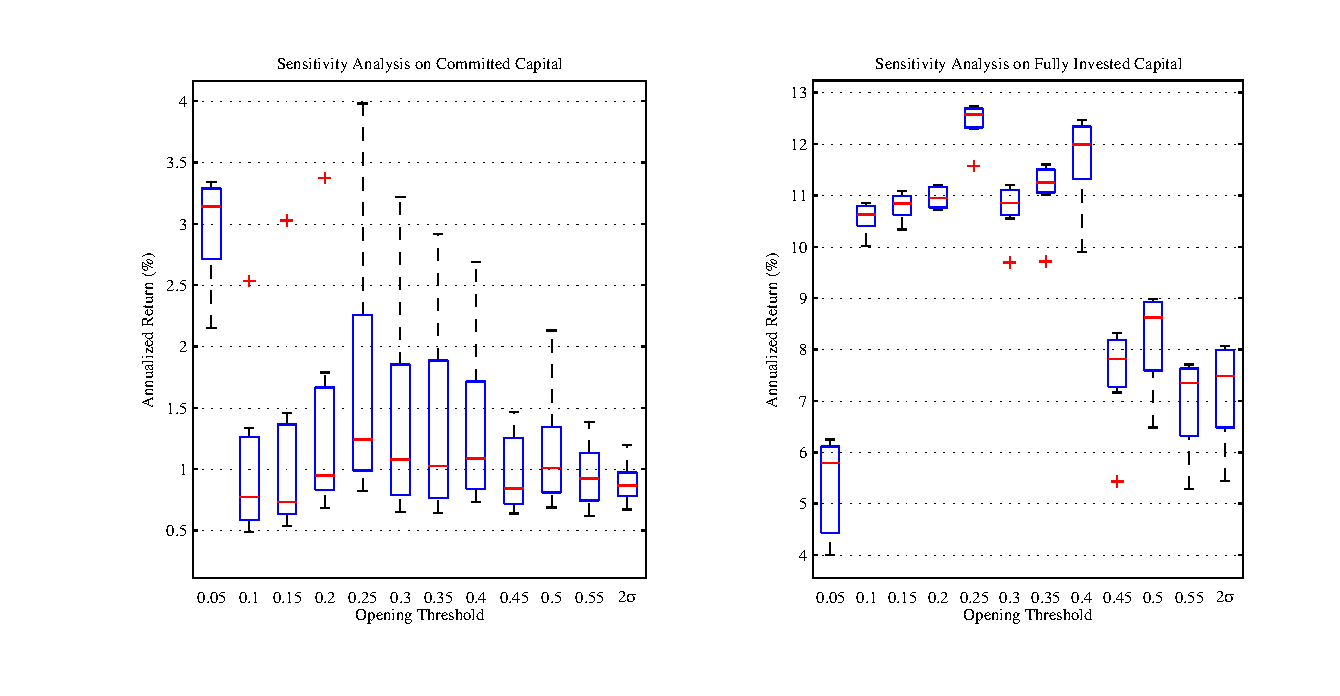
\includegraphics[width=12cm,height=5cm]{Figure1.eps}
		\captionsetup{justification=raggedright,
			singlelinecheck=false
		}
		\caption{\textbf{Annualized returns of pairs trading strategies after costs on committed and fully invested capital}}
		\caption*{\scriptsize These boxplots show annualized returns on committed (left) and fully invested (right) capital after transaction cost to different opening thresholds from July 1991 to December 2015 for Top 5 to Top 35 pairs.}
		\label{fig:fig1}
	\end{figure}

\end{frame}

\begin{frame}
	\frametitle{Risk-Return characteristics}
	
	\begin{figure}[!ht]
		\centering
		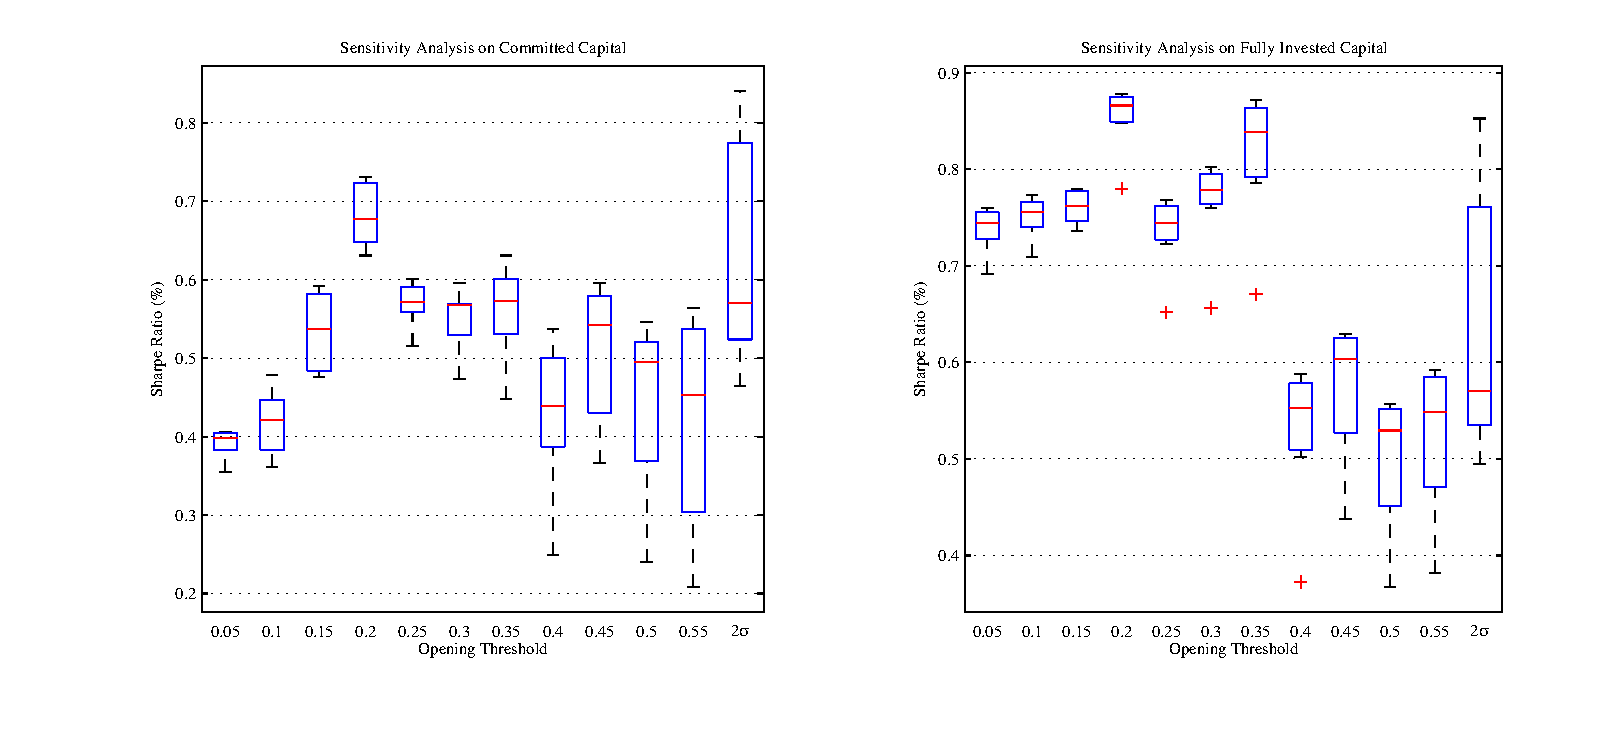
\includegraphics[width=12cm,height=5cm]{Figure2.eps}
		\captionsetup{justification=raggedright,
			singlelinecheck=false
		}
		\caption{\textbf {Sharpe ratio of pairs trading strategies after costs on committed and fully invested capital}}
		\label{fig:fig2}
	\end{figure}
	
\end{frame}

\begin{frame}

\definecolor{corn}{rgb}{0.98, 0.93, 0.36}
\definecolor{celadon}{rgb}{0.67, 0.88, 0.69}
\frametitle{Trading Statistics}

\begin{threeparttable}[H]
	\centering \scriptsize
	\caption{Trading statistics.}
	\begin{tabularx}{\textwidth}{@{\extracolsep{\fill}}p{5cm}p{1cm}p{1cm}p{1cm}p{1cm}@{}}
		\toprule
		\multicolumn{1}{c}{Strategy} & Distance & Mixed Copula \\
		\midrule
		& \multicolumn{4}{c}{\textit{Panel A: Top 5}} \\
		& &  \\
		Average price deviation trigger for opening pairs & 0.0594 & 0.0665  \\
		Total number of pairs opened & \cellcolor{corn} 352   & \cellcolor{corn} 348   \\
		Average number of pairs traded per 6-month & 7.18 & 7.10    \\
		Average number of round-trip trades per pair & 1.44 & 1.42   \\
		~~Standard Deviation & 1.0128 & 1.33   \\
		Average time pairs are open in days & \cellcolor{corn} 50.70 & \cellcolor{corn} 37.70  \\
		~~Standard Deviation & 39.24 & 38.93    \\
		Median time pairs are open in days & \cellcolor{corn} 38.5  & \cellcolor{corn} 19          \\
		& &  \\
		& &  \\
		& \multicolumn{4}{c}{\textit{Panel B: Top20}} \\
		& & \\
		Average price deviation trigger for opening pairs & 0.0681 & 0.0821    \\
		Total number of pairs opened & \cellcolor{celadon} 1312  & \cellcolor{celadon} 749     \\
		Average number of pairs traded per 6-month & 26.78 & 15.29   \\
		Average number of round-trip trades per pair & 1.34 & 0.76  \\
		~Standard Deviation & 0.99 & 0.99    \\
		Average time pairs are open in days & 51.65 & 23.60   \\
		~Standard Deviation & 39.62 & 32.90    \\
		Median time pairs are open in days & 41    & 9           \\
		& & \\
		& \multicolumn{4}{c}{\textit{Panel C: Top 35}} \\
		& & \\
		Average price deviation trigger for opening pairs & 0.0729 & 0.0893   \\
		Total number of pairs opened & 2238  & 941   \\
		Average number of pairs traded per 6-month & 45.68 & 19.20 \\
		Average number of round-trip trades per pair & 1.30 & 0.55   \\
		~Standard Deviation & 1.02 & 0.84   \\
		Average time pairs are open in days & 52.72 &  19.35   \\
		~Standard Deviation & 40.48 & 30.56  \\
		Median time pairs are open in days & 42    & 6           \\
		\bottomrule
	\end{tabularx}%
	\begin{tablenotes}
		\item \textit{Note:} \scriptsize  Trading statistics for portfolio of top 5, 20 and 35 pairs between July 1991 and December 2015 (49 periods). Pairs are formed over a 12-month period according to a minimum-distance (sum of squared deviations) criterion and then traded over the subsequent 6-month period. Average price deviation trigger for opening a pair is calculated as the price difference divided by the average of the prices.
	\end{tablenotes}
	\label{tab:table105}%
\end{threeparttable}%

\end{frame}

\begin{frame}

\definecolor{corn}{rgb}{0.98, 0.93, 0.36}
\definecolor{celadon}{rgb}{0.67, 0.88, 0.69}
\frametitle{Trading Statistics}

\begin{threeparttable}[H]
\centering \scriptsize
\caption{Trading statistics.}
\begin{tabularx}{\textwidth}{@{\extracolsep{\fill}}p{5cm}p{1cm}p{1cm}p{1cm}p{1cm}@{}}
	\toprule
	\multicolumn{1}{c}{Strategy} & Distance & Mixed Copula \\
	\midrule
	& \multicolumn{4}{c}{\textit{Panel C: Top 35}} \\
	& & \\
	Average price deviation trigger for opening pairs & 0.0729 & 0.0893   \\
	Total number of pairs opened & \cellcolor{celadon} 2238  & \cellcolor{celadon} 941   \\
	Average number of pairs traded per six-month period & 45.68 & 19.20 \\
	Average number of round-trip trades per pair & 1.30 & 0.55   \\
	~Standard Deviation & 1.02 & 0.84   \\
	Average time pairs are open in days & 52.72 &  19.35   \\
	~Standard Deviation & 40.48 & 30.56  \\
	Median time pairs are open in days & 42    & 6           \\
	\bottomrule
\end{tabularx}%
\begin{tablenotes}
	\item \textit{Note:} \tiny  Trading statistics for portfolio of top 5, 20 and 35 pairs between July 1991 and December 2015 (49 periods). Pairs are formed over a 12-month period according to a minimum-distance (sum of squared deviations) criterion and then traded over the subsequent 6-month period. Average price deviation trigger for opening a pair is calculated as the price difference divided by the average of the prices.
\end{tablenotes}
\label{tab:table106}%
\end{threeparttable}%

\end{frame}

	\begin{frame}
		
		\definecolor{corn}{rgb}{0.98, 0.93, 0.36}
		\definecolor{celadon}{rgb}{0.67, 0.88, 0.69}
		
		\frametitle{Trading Performance}
			\begin{threeparttable}[H]
			\centering \tiny
			\caption{Excess returns on committed capital of pairs trading strategies on portfolios of Top 5, 20 and 35 pairs after costs. }
			\begin{tabularx}{\textwidth}{@{\extracolsep{\fill}}llllllll@{}}
				\toprule
				Strategy & Mean  & Sharpe & Sortino & t-stat & \% of negative   & MDD1 & MDD2 \\
				& Return (\% ) & ratio &  ratio     &  &  trades     &       &  \\
				\midrule
				\multicolumn{8}{c}{\textbf{Return on Committed Capital}} \\
				\multicolumn{8}{c}{\textit{Panel A - Top 5 pairs}} \\
				&       &       &       &       &       &       &  \\
				Distance & 2.60  & 0.31  & 0.58  & $1.86^{*}$  & 46.98 & 6.73    & 19.62 \\
				Mixed Copula & \cellcolor{corn} 3.98  & \cellcolor{corn} 0.63  & 1.08  & \cellcolor{corn} $3.49^{***}$  & \cellcolor{corn} 41.79 & \cellcolor{corn} 4.36  & \cellcolor{corn} 9.29 \\
				\multicolumn{1}{r}{} & \multicolumn{1}{r}{} & \multicolumn{1}{r}{} & \multicolumn{1}{r}{} & \multicolumn{1}{r}{} & \multicolumn{1}{r}{} & \multicolumn{1}{r}{} & \multicolumn{1}{r}{} \\
				\multicolumn{8}{c}{\textit{Panel B - Top 20 pairs}} \\
				&       &       &       &       &       &       &  \\
				Distance & \cellcolor{celadon} 3.14  & \cellcolor{celadon} 0.65  & 1.13  & $3.32^{***}$  & 48.02 & 3.88  & 9.69 \\
				Mixed Copula  & 1.24  & 0.64  & 1.04  & $3.52^{***}$  & 41.33 & \cellcolor{corn} 2.07  & \cellcolor{corn} 3.43  \\
				\multicolumn{1}{r}{} & \multicolumn{1}{r}{} & \multicolumn{1}{r}{} & \multicolumn{1}{r}{} & \multicolumn{1}{r}{} & \multicolumn{1}{r}{} & \multicolumn{1}{r}{} & \multicolumn{1}{r}{} \\
				\multicolumn{8}{c}{\textit{Panel C - Top 35 pairs}} \\
				&       &       &       &       &       &       &  \\
				Distance & \cellcolor{celadon} 3.12  & \cellcolor{celadon} 0.77  & 1.36  & $3.92^{***}$  & 47.97 & 2.70  & 7.52 \\
				Mixed Copula & 0.82  & 0.73  & 1.19  & $3.95^{***}$  & 41.31 & \cellcolor{corn} 1.18  & \cellcolor{corn} 1.98  \\
				\multicolumn{1}{r}{} & \multicolumn{1}{r}{} & \multicolumn{1}{r}{} & \multicolumn{1}{r}{} & \multicolumn{1}{r}{} & \multicolumn{1}{r}{} & \multicolumn{1}{r}{} & \multicolumn{1}{r}{} \\
				\midrule
				S\&P 500  & 4.36  & \cellcolor{Melon} 0.23  & 0.52  & $1.79^{*}$  & 47.45 & \cellcolor{Melon} 12.42  & \cellcolor{Melon} 46.74  \\
				\bottomrule
			\end{tabularx}%
			\begin{tablenotes}
				\item \textit{Note:} \scriptsize \tiny Summary statistics of the annualized excess returns, annualized Sharpe and Sortino ratios on portfolios of top 5, 20 and 35 pairs between July 1991 and December 2015 (6,173 observations). The t-statistics are computed using Newey-West standard errors with a six-lag correction. The columns labeled MDD1 and MDD2 compute the largest drawdown in terms of maximum percentage drop between two consecutive days and between two days within a period of maximum six months, respectively.
				\item \scriptsize $^{\ast\ast\ast}$, $^{\ast\ast}$, $^{\ast}$  significant at 1\%, 5\% and 10\% levels, respectively.
			\end{tablenotes}
			\label{tab:table101}%
		\end{threeparttable}%

	\end{frame}

\begin{frame}
	\definecolor{corn}{rgb}{0.98, 0.93, 0.36}
	\definecolor{celadon}{rgb}{0.67, 0.88, 0.69}
	\frametitle{Trading Performance}
	\begin{threeparttable}[H]
		\centering \tiny
		\caption{Excess returns on fully invested capital of pairs trading strategies on portfolios of Top 5, 20 and 35 pairs after costs. }
		\begin{tabularx}{\textwidth}{@{\extracolsep{\fill}}llllllll@{}}
			\toprule
			Strategy & Mean  & Sharpe & Sortino & t-stat & \% of negative   & MDD1 & MDD2 \\
			& Return (\% ) & ratio &  ratio     &  &  trades     &       &  \\
			\midrule
			\multicolumn{8}{c}{\textbf{Return on Fully Invested Capital}} \\
			\multicolumn{8}{c}{\textit{Panel A - Top 5 pairs}} \\
			&       &       &       &       &       &       &  \\
			Distance & 4.01  & 0.28  & 0.57  & $1.81^{*}$  & 46.98 & 8.70    & 38.36  \\
			Mixed Copula & 11.58  & 0.78  & 1.43  & $4.26^{***}$  & 41.79 & 9.00  & 25.68 \\
			\multicolumn{1}{r}{} & \multicolumn{1}{r}{} & \multicolumn{1}{r}{} & \multicolumn{1}{r}{} & \multicolumn{1}{r}{} & \multicolumn{1}{r}{} & \multicolumn{1}{r}{} & \multicolumn{1}{r}{} \\
			\multicolumn{8}{c}{\textit{Panel B - Top 20 pairs}} \\
			&       &       &       &       &       &       &  \\
			Distance & 6.07  & 0.66  & 1.19  & $3.55^{***}$  & 48.06 & 5.43  & 20.03 \\
			Mixed Copula  & 12.30  & 0.85  & 1.54  & $4.60^{***}$  & 41.31 & 9.00  & 25.68  \\
			\multicolumn{1}{r}{} & \multicolumn{1}{r}{} & \multicolumn{1}{r}{} & \multicolumn{1}{r}{} & \multicolumn{1}{r}{} & \multicolumn{1}{r}{} & \multicolumn{1}{r}{} & \multicolumn{1}{r}{} \\
			\multicolumn{8}{c}{\textit{Panel C - Top 35 pairs}} \\
			&       &       &       &       &       &       &  \\
			Distance & 5.76  & 0.76  & 1.38  & $4.05^{***}$  & 47.97 & 4.24  & 15.07 \\
			Mixed Copula & 12.73  & 0.88  & 1.59  & $4.73^{***}$  & 41.28 & 9.00  & 25.68  \\
			\multicolumn{1}{r}{} & \multicolumn{1}{r}{} & \multicolumn{1}{r}{} & \multicolumn{1}{r}{} & \multicolumn{1}{r}{} & \multicolumn{1}{r}{} & \multicolumn{1}{r}{} & \multicolumn{1}{r}{} \\
			\bottomrule
		\end{tabularx}%
		\begin{tablenotes}
			\item \scriptsize $^{\ast\ast\ast}$, $^{\ast\ast}$, $^{\ast}$  significant at 1\%, 5\% and 10\% levels, respectively.
		\end{tablenotes}
		\label{tab:table103}%
	\end{threeparttable}%

\end{frame}


\begin{frame}[label=frame5a]
\frametitle{Cumulative excess returns of pairs trading strategies after costs}

\begin{figure}[!ht]
	\centering
	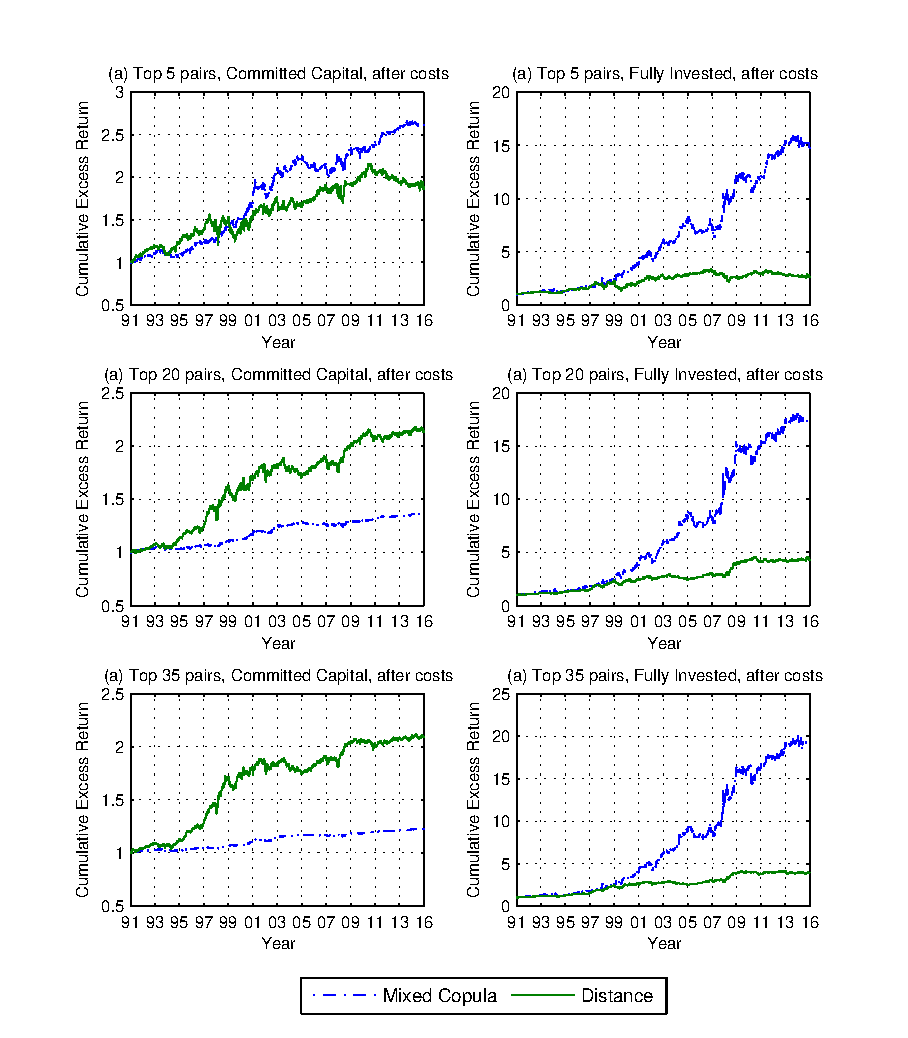
\includegraphics[scale=0.46]{Figure3.eps}
	\captionsetup{justification=raggedright,
		singlelinecheck=false
	}
%	\caption{\textbf{Cumulative excess returns of pairs trading strategies after costs}}
	\caption*{\tiny This figure shows how an investment of \$1 evolves from July 1991 to December 2015 for each of the strategies.}
	\label{fig:fig3}
\end{figure}

\end{frame}


\begin{frame}[label=frame5c]
\frametitle{Kernel density estimation of 5-year rolling window Sharpe ratio after costs}

\begin{figure}[!ht]
	\centering
	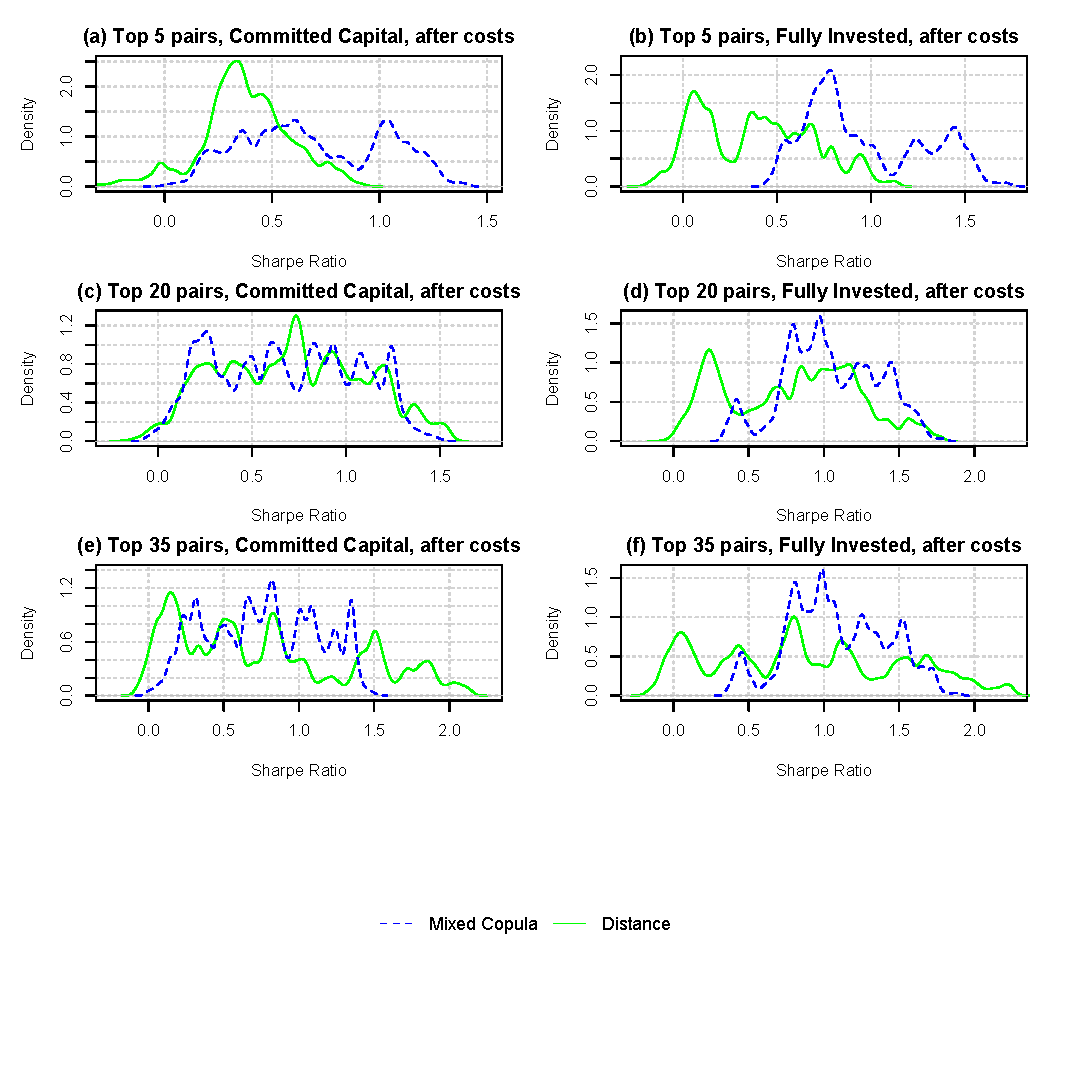
\includegraphics[scale=0.47]{Figure5.eps}
	\captionsetup{justification=raggedright,
		singlelinecheck=false
	}
%	\caption{\textbf{Kernel density estimation of 5-year rolling window Sharpe ratio after costs}}
	\caption*{\tiny  This figure shows how the 5-year rolling window Sharpe ratio densities evolve from July 1996 to December 2015 for each of the strategies with Sheather and Jones (1991)'s bandwidths.}
	\label{fig:fig5}
\end{figure}

\end{frame}


\section{}

\begin{frame}

\setbeamercovered{transparent}

\definecolor{corn}{rgb}{0.98, 0.93, 0.36}
\definecolor{celadon}{rgb}{0.67, 0.88, 0.69}
\frametitle{Systematic Risk Exposure}

\begin{table}
	\centering \srcsize
	\caption{Monthly risk profile of Top 5 pairs: \textcolor{blue}{Fama and French} \textcolor{blue}{(2016)}'s five factors plus Momentum and Long-Term Reversal.}\label{tab:table103}%
	\begin{threeparttable}[!ht]
		\begin{tabularx}{\textwidth}{@{\extracolsep{\fill}} lllllllllll@{}}
			\toprule
			\multicolumn{1}{c}{Strategy} & \multicolumn{1}{c}{Intercept} &  \multicolumn{1}{c}{Rm-Rf} &  \multicolumn{1}{c}{SMB} &  \multicolumn{1}{c}{HML} &  \multicolumn{1}{c}{RMW} &  \multicolumn{1}{c}{CMA} & 
			\multicolumn{1}{c}{Mom} &  \multicolumn{1}{c}{LRev} &  \multicolumn{1}{c}{$R^{2}$} & \multicolumn{1}{c}{$R^{2}_{adj}$} \\
			\midrule
			\multicolumn{11}{c}{\textbf{Section 1: Return on Committed Capital}} \\
			\multicolumn{1}{c}{} & \multicolumn{1}{c}{} & \multicolumn{1}{c}{} & \multicolumn{1}{c}{} & \multicolumn{1}{c}{} & \multicolumn{1}{c}{} & \multicolumn{1}{c}{} & \multicolumn{1}{c}{} & \multicolumn{1}{c}{} & \multicolumn{1}{c}{} & \\
			\multicolumn{1}{c}{Distance} & 0.0025 & 0.0091 & -0.0032 & 0.0113 & 0.0003 & -0.0029 & -0.0107 & -0.0084 & 0.028 & 0.027 \\
			\multicolumn{1}{c}{} & $(1.89)^{*}$ & $(4.22)^{***}$ & (-0.71) & $(2.05)^{**}$ & (0.25) & (-0.18) & $(-4.80)^{***}$ & $(-1.96)^{**}$ & & \\
			\multicolumn{1}{c}{Mixed Copula} &  \cellcolor{corn} 0.0035 & \cellcolor{corn} 0.0052 & -0.0043 & 0.0039 & -0.0035 & 0.0027 & -0.0054 & -0.0057 & \cellcolor{corn} 0.015 &  \cellcolor{corn} 0.014 \\
			\multicolumn{1}{c} {}&  $(3.55)^{***}$ & $(3.68)^{***}$ & $(-1.83)^{*}$ & (1.20) & (-0.99) & (0.63) & $(-2.99)^{***}$ & (-1.57) &  & \\
			
			&       &       &       &       &       &       &       &       &       &       \\
			\midrule
			\multicolumn{11}{c}{\textbf{Section 2: Return on Fully Invested Capital}} \\
			&       &       &       &       &       &       &       &       &       &    \\
			\multicolumn{1}{c}{Distance} & 0.0040 & 0.0170 & -0.0031 & 0.0185 & 0.0049 & -0.0018 & -0.0161 & -0.0150 & 0.025 & 0.024 \\
			\multicolumn{1}{c}{} & $(1.75)^{*}$ & $(4.88)^{***}$ & (-0.45) & $(2.22)^{**}$ & (0.76) & (0.05) & $(-4.30)^{***}$ & $(-1.97)^{**}$ & & \\
			
			\multicolumn{1}{c}{Mixed Copula} & \cellcolor{corn} 0.0098 & \cellcolor{corn} 0.0148 & -0.0084 & 0.0152 & -0.0053 & 0.0087 & -0.0082 & -0.0222 & 0.018 & 0.017 \\
			\multicolumn{1}{c} {}&  $(4.17)^{***}$ & $(3.51)^{***}$ & -1.45 & 1.6355 & -0.60 & 0.75 & $(-2.19)^{**}$ & $(-2.08)^{**}$ & & \\
			\bottomrule
		\end{tabularx}
		\begin{tablenotes}
			\item \tiny $^{\ast\ast\ast}$, $^{\ast\ast}$, $^{\ast}$  significant at 1\%, 5\% and 10\% levels, respectively.
		\end{tablenotes}
	\end{threeparttable}%
\end{table}%

\pause

\begin{itemize}
	\item Alphas are significantly positive and higher than the raw excess returns by about 2-7 bps per month.
	
	\begin{itemize}
		\item Only a small part of the excess returns can be attributed to their exposures to the seven risk determinants
	\end{itemize}
\end{itemize}

%We find that the, of the regressions, indicating that

\end{frame}

\section{}

\begin{frame}[label=frame5b2]
\frametitle{Summary of findings}

\setbeamercovered{transparent}

\begin{enumerate}
	%\setcounter{enumi}{1}
	\justifying
	
	
	\item By capturing linear/nonlinear associations and covering a wider range of possible dependencies structures, the mixed copula strategy outperforms the distance method when the number of trading signals is equiparable, especially after the subprime mortgage crisis.
	
	\pause
	\vspace{0.3cm}
	
	\item The mixed copula pairs trading strategy generates large and significant (at 1\%) abnormal returns.
	
	\pause
		\begin{itemize}
			\item Only a small part of the pairs trading profits can be explained by market portfolio (beta), size (SMB), value (HML), investment (CMA), profitability (RMW), momentum (Mom) and reversal (LRev) based factors.
		\end{itemize}
	
\end{enumerate}

\end{frame}


\begin{frame}
	\frametitle{Extensions}
	
\begin{itemize}
%	\item Varying Threshold
	
%	\vspace{0.3cm}

	\item Copula-based arbitrage for baskets to increase information dependency and measure relative pricing more comprehensively.
	
	%Multivariate models might have the potential to uncovermore from the given data, they however also require an increased amount of computations. Pairs of stocks instead become baskets of stocks
	
	%Create similar 
	\vspace{0.5cm}
	
		\begin{figure}[htbp]
		\centering
		\includegraphics[scale=0.6]{fig4.png}
		\label{fig:fig4}
	\end{figure}

	%\item Vine Copulas (Pair-Copula Constructions)
	
	%\begin{itemize}
		%\item Superior flexibility
	%\end{itemize}
	
\end{itemize}
	
\end{frame}

\begin{frame}
\frametitle{Extensions}

	\begin{figure}[htbp]
	\centering
%	\includegraphics[scale=0.14]{fig3.png}
\includegraphics[scale=0.35]{man_machine2.png}
	\label{fig:fig3}
\end{figure}

\begin{itemize}
		\item Machine Learning and AI-based solutions 
		%(Man + Machine and NOT Man vs Machine) 
		\begin{itemize}
			\item Deep Reinforcement Learning
		\end{itemize}
\vspace{0.3cm}
	\item News Sentiment
	\begin{itemize}
		\item Enhances a pairs-trading strategy using an abnormal news volume and sentiment overlay
		\item Effect of negative news is bigger than positive news
	\end{itemize}
	

	
\end{itemize}

\end{frame}

\begin{frame}

	\centering
	\Large{Thank you! Questions?}
	
\end{frame}

\appendix
\backupbegin

\begin{frame}
\definecolor{corn}{rgb}{0.98, 0.93, 0.36}

\frametitle{Subperiod Analysis}
\begin{threeparttable}[H]
	\centering \tiny
	\caption{Excess returns on committed capital on portfolios of Top 5 pairs after costs. }
	\begin{tabularx}{\textwidth}{@{\extracolsep{\fill}}llll@{}}
		\toprule
		Strategy & Mean  & Sharpe & Sortino \\
		& Return (\% ) & ratio &  ratio     \\
		\midrule
		\multicolumn{4}{c}{\textbf{Return on Committed Capital}} \\
		\multicolumn{4}{c}{\textit{Panel A: 1991-1995}} \\
		&       &       &       \\
		S\&P 500 & 7.17  & 0.72  & 1.30 \\
		Mixed Copula & 2.66  & 0.45  & 0.74 \\
		\multicolumn{1}{r}{} & \multicolumn{1}{r}{} & \multicolumn{1}{r}{} & \multicolumn{1}{r}{} \\
		\multicolumn{4}{c}{\textit{Panel B: 1996-2000}} \\
		&       &       &       \\
		S\&P 500 & 10.03  & 0.51  & 1.01 \\
		Mixed Copula & 6.90  & 1.05  & 1.77 \\
		\multicolumn{1}{r}{} & \multicolumn{1}{r}{} & \multicolumn{1}{r}{} & \multicolumn{1}{r}{} \\
		\multicolumn{4}{c}{\textit{Panel C: 2001-2005}} \\
		&       &       &       \\
		S\&P 500 & -2.28  & \cellcolor{Melon} -0.13  & -0.06 \\
		Mixed Copula & 6.84  & \cellcolor{corn} 0.83  & 1.44 \\
		\multicolumn{1}{r}{} & \multicolumn{1}{r}{} & \multicolumn{1}{r}{} & \multicolumn{1}{r}{} \\
		\multicolumn{4}{c}{\textit{Panel D: 2006:2010}} \\
		&       &       &       \\
		S\&P 500 & -1.71  & \cellcolor{Melon} -0.07  & 0.09 \\
		Mixed Copula & 1.56  & \cellcolor{corn} 0.24  & 0.46 \\
		\multicolumn{1}{r}{} & \multicolumn{1}{r}{} & \multicolumn{1}{r}{} & \multicolumn{1}{r}{} \\
		\multicolumn{4}{c}{\textit{Panel E: 2011:2015}} \\
		&       &       &       \\
		S\&P 500 & 9.91  & 0.61  & 1.09 \\
		Mixed Copula & 2.01  & 0.61  & 1.08 \\
		\multicolumn{1}{r}{} & \multicolumn{1}{r}{} & \multicolumn{1}{r}{} & \multicolumn{1}{r}{} \\
		\bottomrule
	\end{tabularx}%
	\begin{tablenotes}
		\item \scriptsize $^{\ast\ast\ast}$, $^{\ast\ast}$, $^{\ast}$  significant at 1\%, 5\% and 10\% levels, respectively.
	\end{tablenotes}
	\label{tab:table106}%
\end{threeparttable}%

\end{frame}

\begin{frame}

\frametitle{Subperiod Analysis}
\definecolor{corn}{rgb}{0.98, 0.93, 0.36}

\begin{threeparttable}[H]
	\centering \tiny
	\caption{Excess returns on fully invested capital on portfolios of Top 5 pairs after costs. }
	\begin{tabularx}{\textwidth}{@{\extracolsep{\fill}}llll@{}}
		\toprule
		Strategy & Mean  & Sharpe & Sortino \\
		& Return (\% ) & ratio &  ratio     \\
		\midrule
		\multicolumn{4}{c}{\textbf{Return on Fully Invested Capital}} \\
		\multicolumn{4}{c}{\textit{Panel A: 1991-1995}} \\
		&       &       &       \\
		S\&P 500 & 7.17  & 0.72  & 1.30 \\
		Mixed Copula & 7.69  & 0.56  & 1.02 \\
		\multicolumn{1}{r}{} & \multicolumn{1}{r}{} & \multicolumn{1}{r}{} & \multicolumn{1}{r}{} \\
		\multicolumn{4}{c}{\textit{Panel B: 1996-2000}} \\
		&       &       &       \\
		S\&P 500 & 10.03  & 0.51  & 1.01 \\
		Mixed Copula & 19.61  & 1.13  & 1.96 \\
		\multicolumn{1}{r}{} & \multicolumn{1}{r}{} & \multicolumn{1}{r}{} & \multicolumn{1}{r}{} \\
		\multicolumn{4}{c}{\textit{Panel C: 2001-2005}} \\
		&       &       &       \\
		S\&P 500 & -2.28  & \cellcolor{Melon} -0.13  & -0.06 \\
		Mixed Copula & 18.07  & \cellcolor{corn} 1.14  & 2.07 \\
		\multicolumn{1}{r}{} & \multicolumn{1}{r}{} & \multicolumn{1}{r}{} & \multicolumn{1}{r}{} \\
		\multicolumn{4}{c}{\textit{Panel D: 2006:2010}} \\
		&       &       &       \\
		S\&P 500 & -1.71  & \cellcolor{Melon} -0.07  & 0.09 \\
		Mixed Copula & 9.42  & \cellcolor{corn} 0.57  & 1.16 \\
		\multicolumn{1}{r}{} & \multicolumn{1}{r}{} & \multicolumn{1}{r}{} & \multicolumn{1}{r}{} \\
		\multicolumn{4}{c}{\textit{Panel E: 2011:2015}} \\
		&       &       &       \\
		S\&P 500 & 9.91  & 0.61  & 1.09 \\
		Mixed Copula & 3.62  & 0.37  & 0.69 \\
		\multicolumn{1}{r}{} & \multicolumn{1}{r}{} & \multicolumn{1}{r}{} & \multicolumn{1}{r}{} \\
		\bottomrule
	\end{tabularx}%
	\begin{tablenotes}
		\item \scriptsize $^{\ast\ast\ast}$, $^{\ast\ast}$, $^{\ast}$  significant at 1\%, 5\% and 10\% levels, respectively.
	\end{tablenotes}
	\label{tab:table107}%
\end{threeparttable}%

\end{frame}

\begin{frame}
\definecolor{corn}{rgb}{0.98, 0.93, 0.36}

\frametitle{Subperiod Analysis}
\begin{threeparttable}[H]
	\centering \tiny
	\caption{Excess returns on committed capital on portfolios of Top 20 pairs after costs. }
	\begin{tabularx}{\textwidth}{@{\extracolsep{\fill}}llll@{}}
		\toprule
		Strategy & Mean  & Sharpe & Sortino \\
		& Return (\% ) & ratio &  ratio     \\
		\midrule
		\multicolumn{4}{c}{\textbf{Return on Committed Capital}} \\
		\multicolumn{4}{c}{\textit{Panel A: 1991-1995}} \\
		&       &       &       \\
		S\&P 500 & 7.17  & 0.72  & 1.30 \\
		Mixed Copula & 0.93  & 0.46  & 0.70 \\
		\multicolumn{1}{r}{} & \multicolumn{1}{r}{} & \multicolumn{1}{r}{} & \multicolumn{1}{r}{} \\
		\multicolumn{4}{c}{\textit{Panel B: 1996-2000}} \\
		&       &       &       \\
		S\&P 500 & 10.03  & 0.51  & 1.01 \\
		Mixed Copula & 1.67  & 0.84  & 1.37 \\
		\multicolumn{1}{r}{} & \multicolumn{1}{r}{} & \multicolumn{1}{r}{} & \multicolumn{1}{r}{} \\
		\multicolumn{4}{c}{\textit{Panel C: 2001-2005}} \\
		&       &       &       \\
		S\&P 500 & -2.28  & \cellcolor{Melon} -0.13  & -0.06 \\
		Mixed Copula & 2.43  & \cellcolor{corn} 1.09  & 1.86 \\
		\multicolumn{1}{r}{} & \multicolumn{1}{r}{} & \multicolumn{1}{r}{} & \multicolumn{1}{r}{} \\
		\multicolumn{4}{c}{\textit{Panel D: 2006:2010}} \\
		&       &       &       \\
		S\&P 500 & -1.71  & \cellcolor{Melon} -0.07  & 0.09 \\
		Mixed Copula & 0.49  & \cellcolor{corn} 0.22  & 0.38 \\
		\multicolumn{1}{r}{} & \multicolumn{1}{r}{} & \multicolumn{1}{r}{} & \multicolumn{1}{r}{} \\
		\multicolumn{4}{c}{\textit{Panel E: 2011:2015}} \\
		&       &       &       \\
		S\&P 500 & 9.91  & 0.61  & 1.09 \\
		Mixed Copula & 0.70  & 0.77  & 1.30 \\
		\multicolumn{1}{r}{} & \multicolumn{1}{r}{} & \multicolumn{1}{r}{} & \multicolumn{1}{r}{} \\
		\bottomrule
	\end{tabularx}%
	\begin{tablenotes}
		\item \scriptsize $^{\ast\ast\ast}$, $^{\ast\ast}$, $^{\ast}$  significant at 1\%, 5\% and 10\% levels, respectively.
	\end{tablenotes}
	\label{tab:table108}%
\end{threeparttable}%

\end{frame}

\begin{frame}

\frametitle{Subperiod Analysis}
\definecolor{corn}{rgb}{0.98, 0.93, 0.36}

\begin{threeparttable}[H]
\centering \tiny
\caption{Excess returns on fully invested capital on portfolios of Top 20 pairs after costs. }
\begin{tabularx}{\textwidth}{@{\extracolsep{\fill}}llll@{}}
	\toprule
	Strategy & Mean  & Sharpe & Sortino \\
	& Return (\% ) & ratio &  ratio     \\
	\midrule
	\multicolumn{4}{c}{\textbf{Return on Fully Invested Capital}} \\
	\multicolumn{4}{c}{\textit{Panel A: 1991-1995}} \\
	&       &       &       \\
	S\&P 500 & 7.17  & 0.72  & 1.30 \\
	Mixed Copula & 8.18  & 0.63  & 1.10 \\
	\multicolumn{1}{r}{} & \multicolumn{1}{r}{} & \multicolumn{1}{r}{} & \multicolumn{1}{r}{} \\
	\multicolumn{4}{c}{\textit{Panel B: 1996-2000}} \\
	&       &       &       \\
	S\&P 500 & 10.03  & 0.51  & 1.01 \\
	Mixed Copula & 18.48  & 1.08  & 1.85 \\
	\multicolumn{1}{r}{} & \multicolumn{1}{r}{} & \multicolumn{1}{r}{} & \multicolumn{1}{r}{} \\
	\multicolumn{4}{c}{\textit{Panel C: 2001-2005}} \\
	&       &       &       \\
	S\&P 500 & -2.28  & \cellcolor{Melon} -0.13  & -0.06 \\
	Mixed Copula & 21.07  & \cellcolor{corn} 1.34  & 2.42 \\
	\multicolumn{1}{r}{} & \multicolumn{1}{r}{} & \multicolumn{1}{r}{} & \multicolumn{1}{r}{} \\
	\multicolumn{4}{c}{\textit{Panel D: 2006:2010}} \\
	&       &       &       \\
	S\&P 500 & -1.71  & \cellcolor{Melon} -0.07  & 0.09 \\
	Mixed Copula & 12.09  & \cellcolor{corn} 0.74  & 1.48 \\
	\multicolumn{1}{r}{} & \multicolumn{1}{r}{} & \multicolumn{1}{r}{} & \multicolumn{1}{r}{} \\
	\multicolumn{4}{c}{\textit{Panel E: 2011:2015}} \\
	&       &       &       \\
	S\&P 500 & 9.91  & 0.61  & 1.09 \\
	Mixed Copula & 2.33  & 0.25  & 0.49 \\
	\multicolumn{1}{r}{} & \multicolumn{1}{r}{} & \multicolumn{1}{r}{} & \multicolumn{1}{r}{} \\
	\bottomrule
\end{tabularx}%
\begin{tablenotes}
	\item \scriptsize $^{\ast\ast\ast}$, $^{\ast\ast}$, $^{\ast}$  significant at 1\%, 5\% and 10\% levels, respectively.
\end{tablenotes}
\label{tab:table109}%
\end{threeparttable}%

\end{frame}

\begin{frame}
\definecolor{corn}{rgb}{0.98, 0.93, 0.36}

\frametitle{Subperiod Analysis}
\begin{threeparttable}[H]
	\centering \tiny
	\caption{Excess returns on committed capital on portfolios of Top 35 pairs after costs. }
	\begin{tabularx}{\textwidth}{@{\extracolsep{\fill}}llll@{}}
		\toprule
		Strategy & Mean  & Sharpe & Sortino \\
		& Return (\% ) & ratio &  ratio     \\
		\midrule
		\multicolumn{4}{c}{\textbf{Return on Committed Capital}} \\
		\multicolumn{4}{c}{\textit{Panel A: 1991-1995}} \\
		&       &       &       \\
		S\&P 500 & 7.17  & 0.72  & 1.30 \\
		Mixed Copula & 0.70  & 0.60  & 0.93 \\
		\multicolumn{1}{r}{} & \multicolumn{1}{r}{} & \multicolumn{1}{r}{} & \multicolumn{1}{r}{} \\
		\multicolumn{4}{c}{\textit{Panel B: 1996-2000}} \\
		&       &       &       \\
		S\&P 500 & 10.03  & 0.51  & 1.01 \\
		Mixed Copula & 0.99  & 0.84  & 1.37 \\
		\multicolumn{1}{r}{} & \multicolumn{1}{r}{} & \multicolumn{1}{r}{} & \multicolumn{1}{r}{} \\
		\multicolumn{4}{c}{\textit{Panel C: 2001-2005}} \\
		&       &       &       \\
		S\&P 500 & -2.28  & \cellcolor{Melon} -0.13  & -0.06 \\
		Mixed Copula & 1.59  & \cellcolor{corn} 1.23  & 2.11 \\
		\multicolumn{1}{r}{} & \multicolumn{1}{r}{} & \multicolumn{1}{r}{} & \multicolumn{1}{r}{} \\
		\multicolumn{4}{c}{\textit{Panel D: 2006:2010}} \\
		&       &       &       \\
		S\&P 500 & -1.71  & \cellcolor{Melon} -0.07  & 0.09 \\
		Mixed Copula & 0.35  & \cellcolor{corn} 0.28  & 0.46 \\
		\multicolumn{1}{r}{} & \multicolumn{1}{r}{} & \multicolumn{1}{r}{} & \multicolumn{1}{r}{} \\
		\multicolumn{4}{c}{\textit{Panel E: 2011:2015}} \\
		&       &       &       \\
		S\&P 500 & 9.91  & 0.61  & 1.09 \\
		Mixed Copula & 0.50  & 0.86  & 1.56 \\
		\multicolumn{1}{r}{} & \multicolumn{1}{r}{} & \multicolumn{1}{r}{} & \multicolumn{1}{r}{} \\
		\bottomrule
	\end{tabularx}%
	\begin{tablenotes}
		\item \scriptsize $^{\ast\ast\ast}$, $^{\ast\ast}$, $^{\ast}$  significant at 1\%, 5\% and 10\% levels, respectively.
	\end{tablenotes}
	\label{tab:table110}%
\end{threeparttable}%

\end{frame}

\begin{frame}

\frametitle{Subperiod Analysis}
\definecolor{corn}{rgb}{0.98, 0.93, 0.36}

\begin{threeparttable}[H]
\centering \tiny
\caption{Excess returns on fully invested capital on portfolios of Top 35 pairs after costs. }
\begin{tabularx}{\textwidth}{@{\extracolsep{\fill}}llll@{}}
	\toprule
	Strategy & Mean  & Sharpe & Sortino \\
	& Return (\% ) & ratio &  ratio     \\
	\midrule
	\multicolumn{4}{c}{\textbf{Return on Fully Invested Capital}} \\
	\multicolumn{4}{c}{\textit{Panel A: 1991-1995}} \\
	&       &       &       \\
	S\&P 500 & 7.17  & 0.72  & 1.30 \\
	Mixed Copula & 8.50  & 0.65  & 1.14 \\
	\multicolumn{1}{r}{} & \multicolumn{1}{r}{} & \multicolumn{1}{r}{} & \multicolumn{1}{r}{} \\
	\multicolumn{4}{c}{\textit{Panel B: 1996-2000}} \\
	&       &       &       \\
	S\&P 500 & 10.03  & 0.51  & 1.01 \\
	Mixed Copula & 19.10  & 1.12  & 1.93 \\
	\multicolumn{1}{r}{} & \multicolumn{1}{r}{} & \multicolumn{1}{r}{} & \multicolumn{1}{r}{} \\
	\multicolumn{4}{c}{\textit{Panel C: 2001-2005}} \\
	&       &       &       \\
	S\&P 500 & -2.28  & \cellcolor{Melon} -0.13  & -0.06 \\
	Mixed Copula & 21.81  & \cellcolor{corn} 1.38  & 2.50 \\
	\multicolumn{1}{r}{} & \multicolumn{1}{r}{} & \multicolumn{1}{r}{} & \multicolumn{1}{r}{} \\
	\multicolumn{4}{c}{\textit{Panel D: 2006:2010}} \\
	&       &       &       \\
	S\&P 500 & -1.71  & \cellcolor{Melon} -0.07  & 0.09 \\
	Mixed Copula & 12.39  & \cellcolor{corn} 0.76  & 1.51 \\
	\multicolumn{1}{r}{} & \multicolumn{1}{r}{} & \multicolumn{1}{r}{} & \multicolumn{1}{r}{} \\
	\multicolumn{4}{c}{\textit{Panel E: 2011:2015}} \\
	&       &       &       \\
	S\&P 500 & 9.91  & 0.61  & 1.09 \\
	Mixed Copula & 2.56  & 0.27  & 0.53 \\
	\multicolumn{1}{r}{} & \multicolumn{1}{r}{} & \multicolumn{1}{r}{} & \multicolumn{1}{r}{} \\
	\bottomrule
\end{tabularx}%
\begin{tablenotes}
	\item \scriptsize $^{\ast\ast\ast}$, $^{\ast\ast}$, $^{\ast}$  significant at 1\%, 5\% and 10\% levels, respectively.
\end{tablenotes}
\label{tab:table111}%
\end{threeparttable}%

\end{frame}

\backupend

\end{document}







